


%% HEAD SUPERTABULAR %%
\rowcolors{1}{light-gray}{white}
\newlength{\Li}\settowidth{\Li}{\textbf{Decimal}}
\newlength{\Liii}\settowidth{\Liii}{(bootstrap  )}
\newlength{\Lii}\settowidth{\Lii}{SCHEDULETABLE\_AUTOSTART }
\tablefirsthead{ \textbf{Decimal Value} & \textbf{bit 5}  & \textbf{bit 4} & \textbf{bit 3} & \textbf{bit 2} & \textbf{bit 1} & \textbf{bit 0} & \textbf{Meaning} \\ \hline }
\tablehead{ \rowcolor{white} \rowcolors{1}{light-gray}{white} \textbf{Decimal Value} & \textbf{bit 5}  & \textbf{bit 4} & \textbf{bit 3} & \textbf{bit 2} & \textbf{bit 1} & \textbf{bit 0} & \textbf{Meaning} \\ \hline  }
\tabletail{ \hline } 
\tablelasttail{}


\chapter{Schedule Table Implementation}

\section{The States of a Schedule Table}

A schedule table always has a defined state. States include those found at page 42 of the AUTOSAR specifications 3.1 and others states used for internal management.

Indeed, \textbf{bit 1} is the "autostart" bit. It's used when autostarted schedule tables have been declared in the OIL file. Goil generates schedule tables with SCHEDULETABLE\_AUTOSTART\_X (X can be RELATIVE, ABSOLUTE or SYNCHRON) state. At startup (in tpl\_init\_os()), the system starts autostarted schedule tables and resets the \textbf{bit 1}.

\textbf{bit 4} is the "bootstrap" bit. It's used when the first expiry point of a schedule table is dated in more than \textbf{OsCounterMaxAllowedValue} ticks from the current date \footnote{As the \textit{$<$offset$>$} parameter of StartScheduleTableRel() cannot be greater than \textbf{OsCounterMaxAllowedValue} minus the \textbf{InitialOffset} of the schedule table (OS276), the first expiry point cannot be in more than \textbf{OsCounterMaxAllowedValue} ticks from the current date. Thus the "bootstrap" bit can set by StartScheduleTableAbs() only.}. It can happen when :
	\begin{itemize}
	\item the schedule table start ($<$tick\_val$>$) is after the current date and the first expiry point comes between the current date and $<$tick\_val$>$
	\item $<$tick\_val$>$ is before the current date and the first expiry point comes after the current date
	\end{itemize}

Figure \ref{fig:bootstrapexample} below shows a bootstrap example for the first item.

\begin{figure}[H] %  figure placement: here, top, bottom, or page
   \centering
   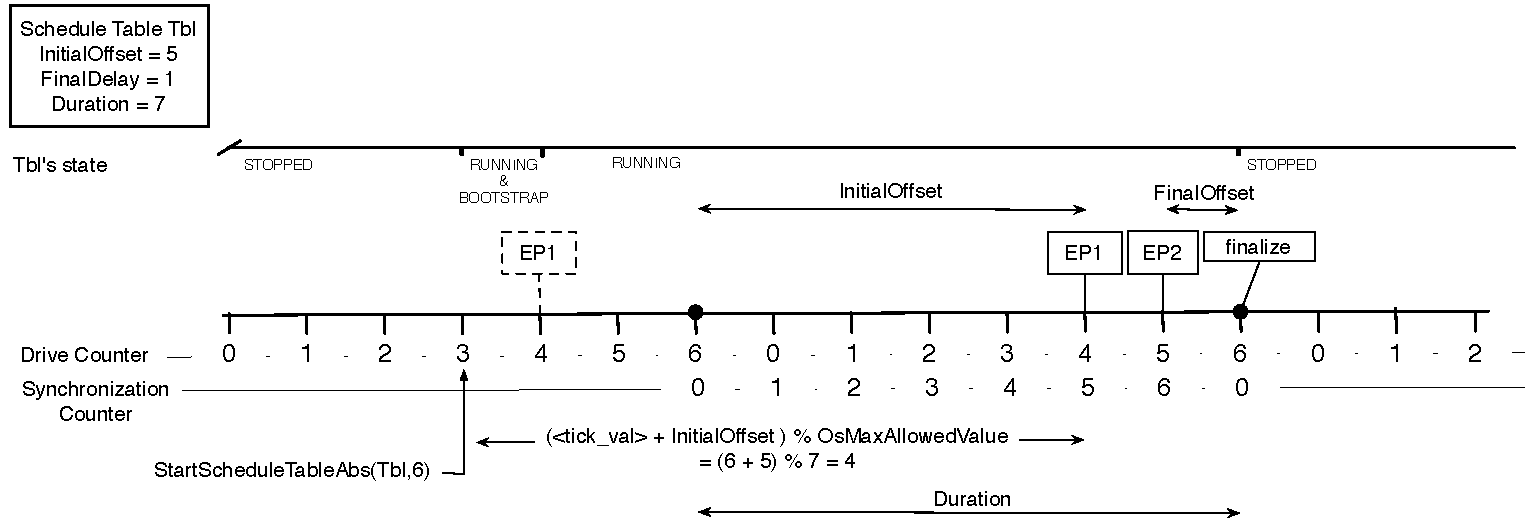
\includegraphics[width=6in]{pictures/BootstrapExample.pdf}  
   \caption{Bootstrap example}
   \label{fig:bootstrapexample}
\end{figure} 

\textbf{bit 5} is the "asynchronous" bit. It tells the system that the schedule table is in asynchronous mode.\\
Thus, the different states of a schedule table are described in Table \ref{schedtablestates} below.


\begin{table}[H]
\begin{center}
\topcaption{\textcolor{white}{q}States of a schedule table } % Latex is weird, the table goes on the next page without the "\textcolor{white}{q}"
\begin{supertabular}{p{\Li}|c|c|c|c|c|c|p{\Lii}|} 
0	& 0	& 0	& 0 	& 0	& 0	& 0	& SCHEDULETABLE\_STOPPED  \\ 
1	& 0	& 0	& 0 	& 0	& 0	& 1	& SCHEDULETABLE\_RUNNING  \\ 
5	& 0	& 0	& 0 	& 1	& 0	& 1	& SCHEDULETABLE\_NEXT  \\  
9	& 0	& 0	& 1 	& 0	& 0	& 1	& SCHEDULETABLE\_WAITING  \\  
13	& 0	& 0	& 1 	& 1	& 0	& 1	& SCHEDULETABLE\_RUNNING\_AND\_SYNCHRONOUS \\ \hline \hline
6	& 0	& 0	& 0 	& 1	& 1	& 0	& SCHEDULETABLE\_AUTOSTART \_ABSOLUTE  \\ 
10	& 0	& 0	& 1 	& 0	& 1	& 0	& SCHEDULETABLE\_AUTOSTART \_RELATIVE  \\  
14	& 0	& 0	& 1 	& 1	& 1	& 0	& SCHEDULETABLE\_AUTOSTART \_SYNCHRON  \\  \hline \hline
16	& 0	& 1	& 0 	& 0	& 0	& 0	& SCHEDULETABLE\_BOOTSTRAP \\ 
32	& 1	& 0	& 0 	& 0	& 0	& 0	& SCHEDULETABLE\_ASYNC  \\ 
\end{supertabular} 
\end{center}
\label{schedtablestates}
\end{table}

Figure \ref{fig:STstates} shows how a schedule table goes from state to state.

\begin{figure}[H] %  figure placement: here, top, bottom, or page
   \centering
   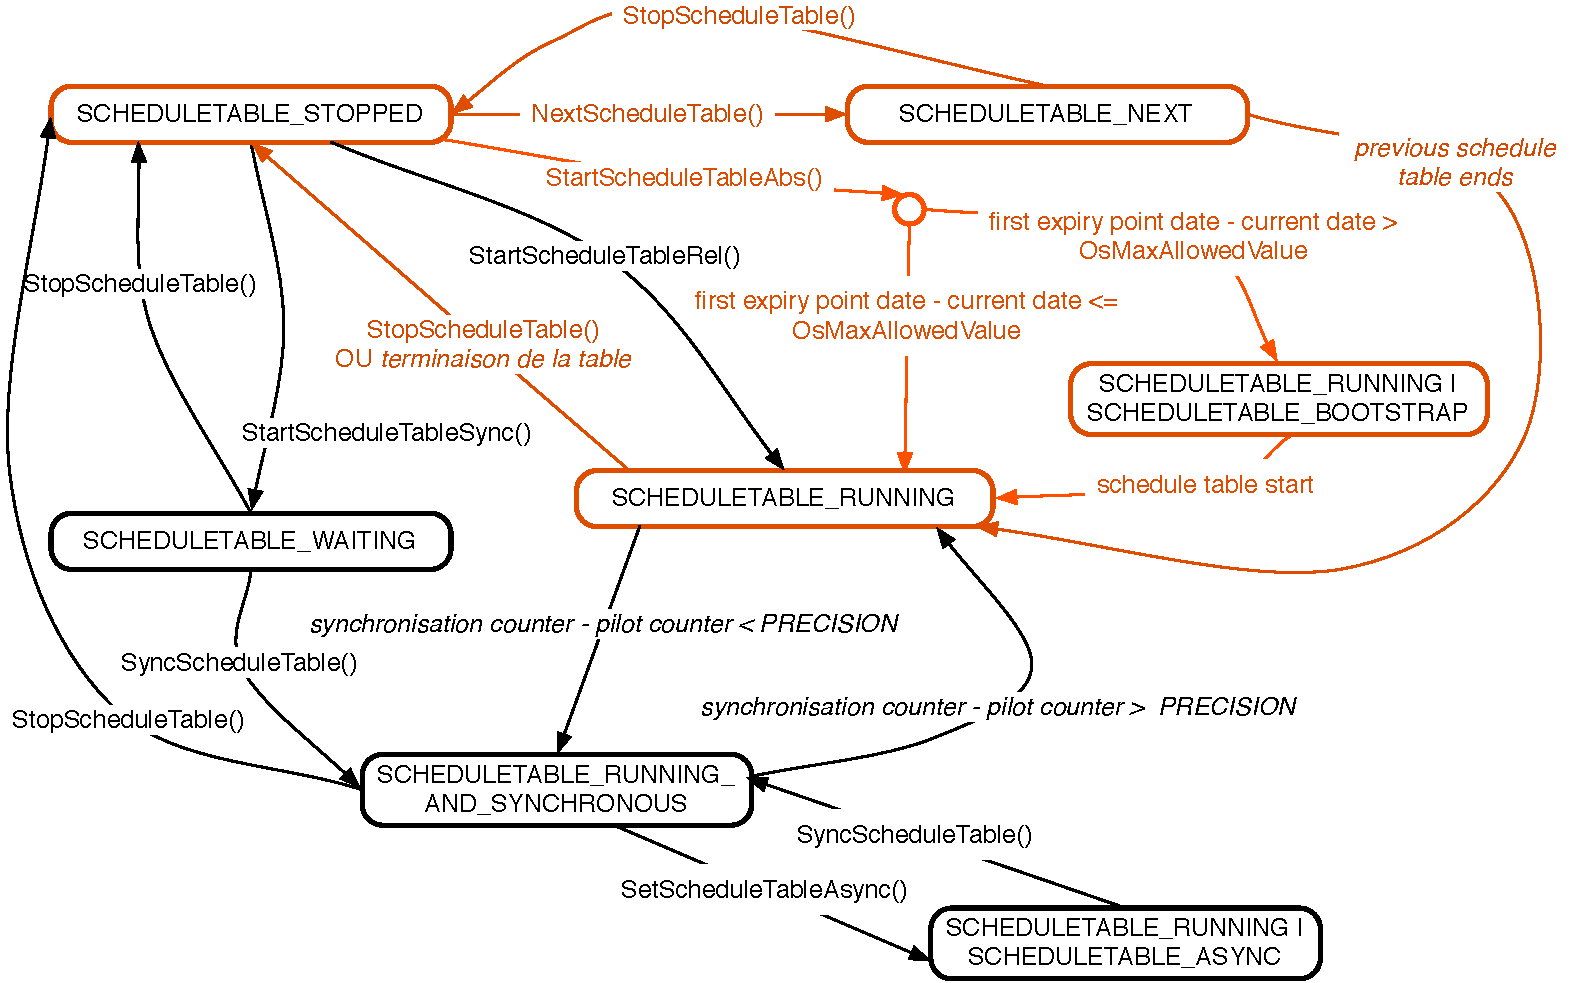
\includegraphics[width=6in]{pictures/STstates.pdf}  
   \caption{States of a schedule table in Trampoline.}
   \label{fig:STstates}
\end{figure} 
	
\section{Processing a Schedule Table}

GOIL generates one expiry point more than the number of expiry point delared by the User : the "finalize" expiry point (see Figure \ref{fig:bootstrapexample}). Indeed, the RUNNING state of a "nexted" schedule table should be set at the finalize expiry point, thus, this expiry point is inserted to do it. For a periodic schedule table, the finalize expiry point helps to launch the first expiry point of the next period.

To process a \textbf{synchronized} schedule table, the schedule table's state has to be updated every expiry point and the next expiry point has to be adjusted according to the schedule table's deviation.

A schedule table is a time object, like an alarm. \textit{tpl\_processing\_scheduletable()} is called by each expiry point (before activating a task, setting an event or finalizing a schedule table via \textit{tpl\_finalize\_expiry\_point()}) . The state machine of this function is shown in the Figure \ref{fig:STprocessingTplProcess}.

\begin{figure}[H] %  figure placement: here, top, bottom, or page
   \centering
   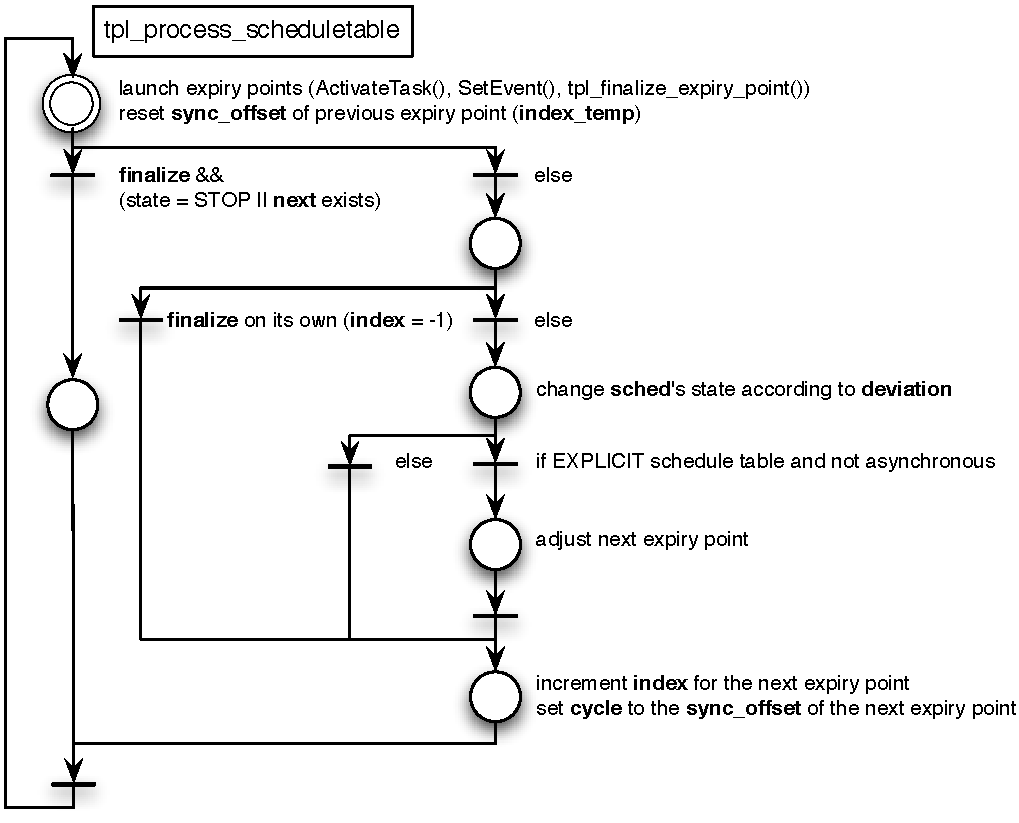
\includegraphics[width=5in]{pictures/STprocessingTplProcess.pdf}  
   \caption{tpl_process_scheduletable's state machine.}
   \label{fig:STprocessingTplProcess}
\end{figure} 

\begin{figure}[H] %  figure placement: here, top, bottom, or page
   \centering
   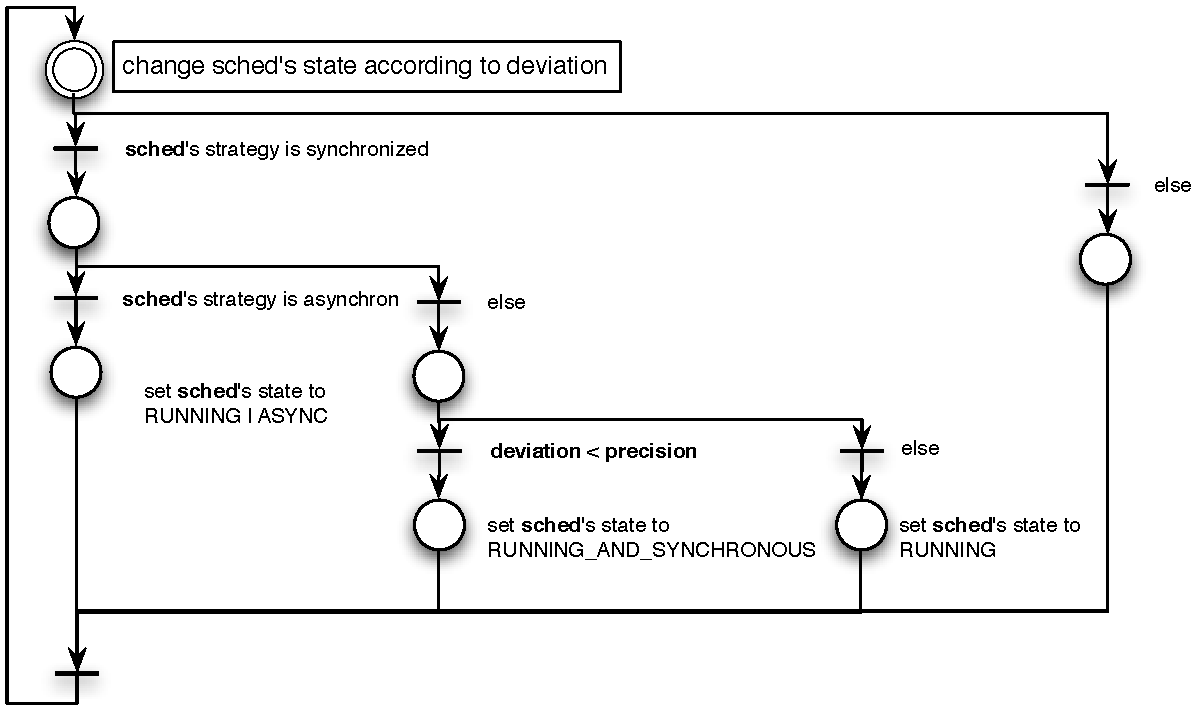
\includegraphics[width=5in]{pictures/STprocessingChangeState.pdf}  
   \label{fig:STprocessingChangeState}
\end{figure}

\textit{tpl\_finalize\_expoiry\_point()} state machine is shown in Figure \ref{fig:STprocessingTplFinalize} below.

\begin{figure}[H] %  figure placement: here, top, bottom, or page
   \centering
   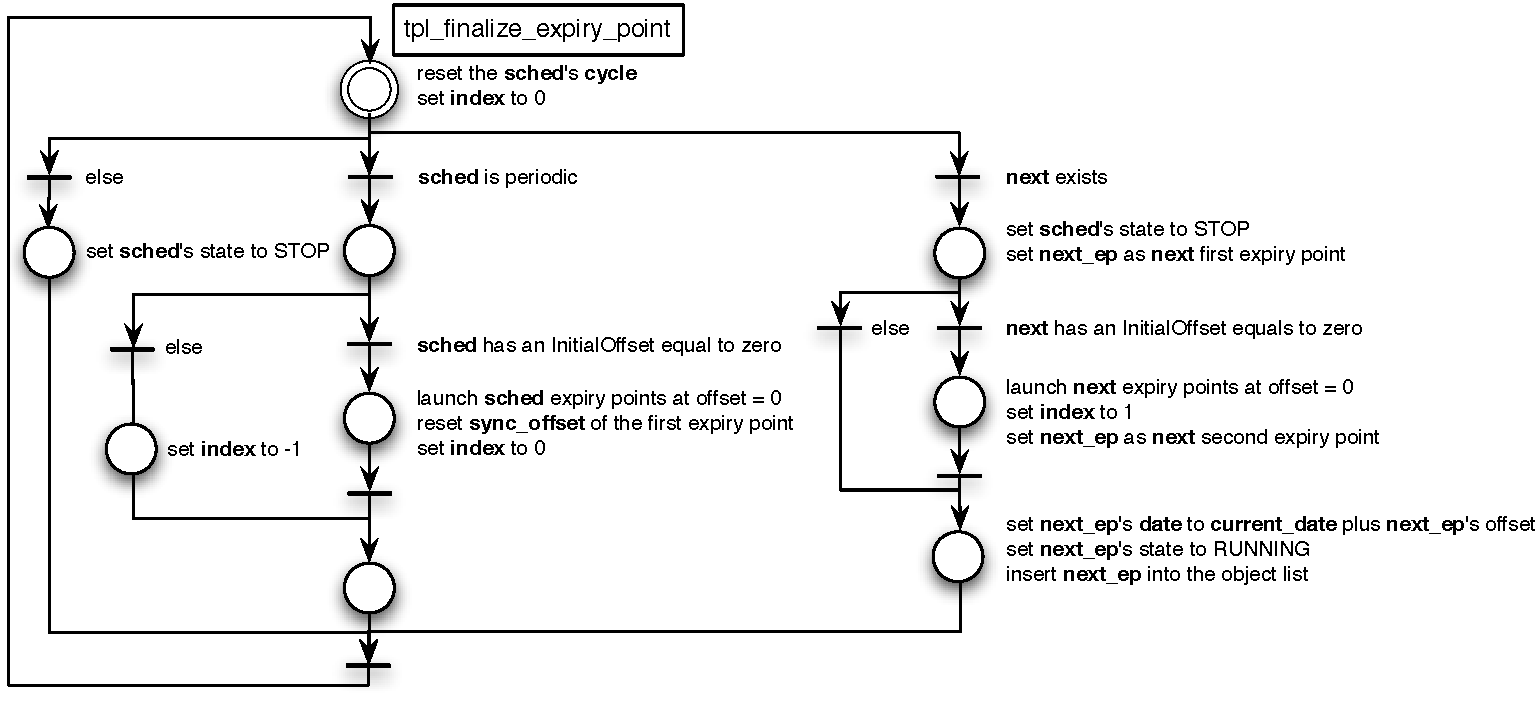
\includegraphics[width=7in]{pictures/STprocessingTplFinalize.pdf}  
   \caption{tpl_finalize_expiry_point's state machine.}
   \label{fig:STprocessingTplFinalize}
\end{figure} 
















